\section{Konfiguracja}
Konfiguracja wszystkich peryferiów wymaganych do uruchomienia układu została przeprowadzona w programie \textit{CubeMX}. Następnie na jej podstawie wygenerowano projekt do dalszego rozwijania w środowisku \textit{Eclipse}. Na rysunku \ref{stmPorty} przedstawiono konfiguracje poszczególnych portów mikrokontrolera.

\begin{figure}[h!]
	\centering
	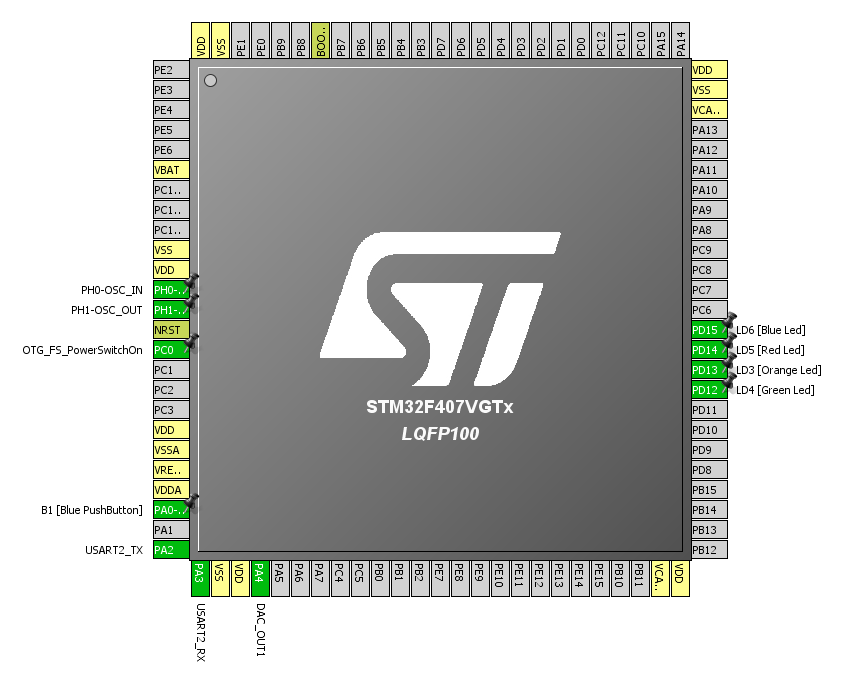
\includegraphics[scale = 0.4]{fig/stmPorty.png}
	\caption		
	{Konfiguracja portów mikrokontrolera Stm32 w programie \textit{CubeMX}.}
	\label{stmPorty}
\end{figure}


\subsection{Konfiguracja timerów}
Do cyklicznego generowania kolejnych próbek sygnału wyjściowego wykorzystano przerwanie od Timera nr 11. Licznik skonfigurowano tak aby generował przerwanie z częstotliwością 100 kHz. Na rysunku \ref{timer11} pokazany jest panel konfiguracyjny timer-a z programu \textit{CubeMX}, natomiast na rysunku \ref{stmclock} konfiguracja sygnałów zegarowych w całym układzie.  

\begin{figure}[h!]
	\centering
	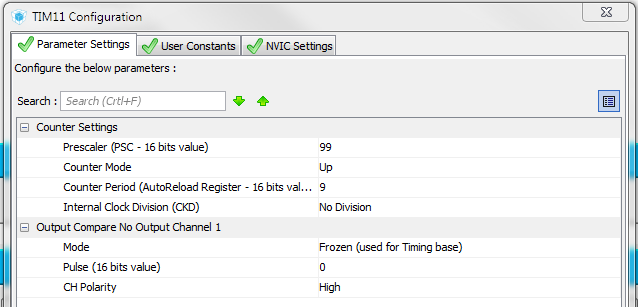
\includegraphics[scale = 0.8]{fig/timer11.png}
	\caption		
	{Przykład konfiguracji timera 11.}
	\label{timer11}
\end{figure}

\begin{figure}[h!]
	\centering
	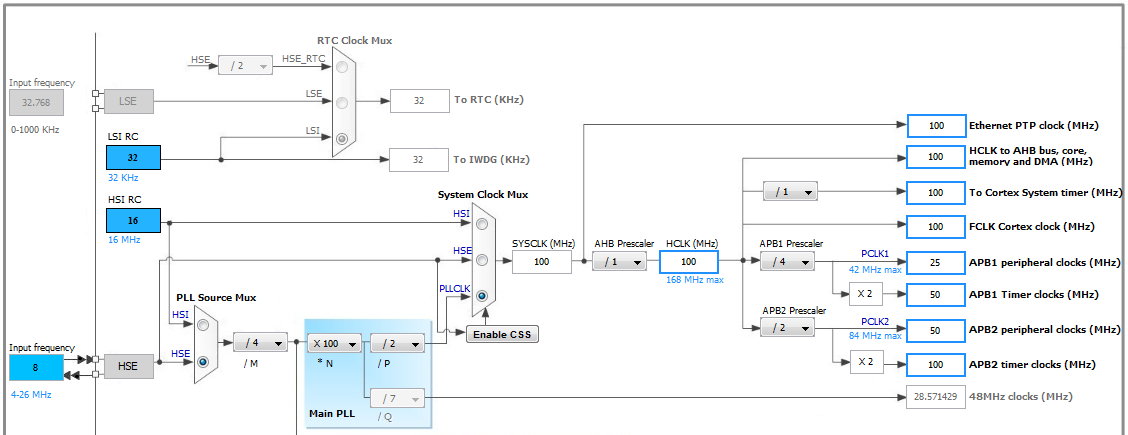
\includegraphics[scale = 0.5]{fig/clock.png}
	\caption		
	{Konfiguracja sygnałów zegarowych w układzie.}
	\label{stmclock}
\end{figure}

\subsection{Konfiguracja przetwornika DAC}
Przetwornik DAC został skonfigurowany w trybie 12 bitowym, a do generacji sygnału wyjściowego wykorzystywany był pierwszy kanał przetwornika na pinie PA4. Z racji na ograniczoną rozdzielczość przetwornika zdecydowano się na ograniczenie wartości amplitudy generowanego sygnału do $\pm 50$. Ponieważ wartości poszczególnych punktów postaci czasowej sygnału mogą przyjmować wartości zarówno dodatnie jak i ujemne, to przyjęto, że wartość zero odpowiada liczbie 2048 wpisanej do rejestru przetwornika.   
\subsection{Konfiguracja portu szeregowego}

Do przesyłania danych z komputera do mikrokontrolera wykorzystany został protokół szeregowy \textit{RS232}. Parametry charakteryzujące transmisję podane są w tabeli \ref{tab_rs232}.

\begin{table}[h]
	\caption{Parametry portu szeregowego.}
	\label{tab_rs232}
	\centering
	
	\begin{tabular}{|c|c|}
		\hline
		\textbf{Parametr} & \textbf{Wartość}\\
		\hline
		Prędkość transmisji & 115200 Bitów/s \\
		\hline
		Długość słowa & 8 bitów \\
		\hline
		Bit parzystości & - \\
		\hline
		Bit stopu & 1 \\
		\hline
	\end{tabular}
\end{table}   